\documentclass[11pt]{article}
\usepackage[margin=1in]{geometry}

\usepackage{amsmath}
\usepackage{listings}
\usepackage{graphicx}
\usepackage{pythonhighlight}
\usepackage{subfig}
\usepackage{caption}
\usepackage{float}
\usepackage{subfig}

\author{Francesco Saverio Zuppichini}
\title{Machine Learning - Assignment 1}
\begin{document}
\maketitle

\section{The Perceptron}
\subsection{Question 1}
\subsubsection{Vectorized equations}
Equation \ref{eq:vectorized_perceptron} shows the vectorised equation for a single perceptron

\begin{equation}
\label{eq:vectorized_perceptron}
output = XW + b
\end{equation}
Where $X = {x_1, ... x_n}$, $W = {w_1, ..., w_n}$. We denote $y$ the output of the perceptron

\subsubsection{Mean Squared Error}
Equation \ref{eq: MSE_perceptron} denotes the Mean Square Error function for our single perceptron
\begin{equation}
\label{eq: MSE_perceptron}
	E(w) = \frac{1}{N}\sum_{i = 1}^N(\underbrace{y(x_i,w_i)}_{\text{predicted}} - \underbrace{t_i}_{\text{actual}})^2)
\end{equation}
One trick that is usual done is to multiply equation $(2)$ by $\frac{1}{2}$, so when we take the derivative the $2$ goes away. This is called One Half Mean Squared Error.

\subsubsection{Derivate of the error with respect to the weights}
In order to reduce our error function and adjust each weight we need to compute the first derivati with respect to the weights. We will use the modified version of equation $(2)$ called One Half Mean Squared Error.
\begin{equation}
\frac{\delta E}{\delta w_i}	= y - t
\end{equation}
\subsubsection{Compute the new weight values after one step using a learning rate of 0.02}
Since it was not specified that the calculation must be done by hand, we called \texttt{train\_one\_step} in order to compute the new weights, as follow
\begin{python}
X,T = get_part1_data()
p = Perceptron()
train_one_step(p,0.02,X,T)
print(p.var['W']) //output weights the values	
print(p.var['b']) //output the new bias value
\end{python}
Where the new weights and bias are
$$W_{k + 1} = \begin{pmatrix}
 0.43963636 \\
 -0.75109091
\end{pmatrix}, b_{k+1} = \begin{pmatrix}
	1.95218181818
\end{pmatrix}$$
\subsubsection{Gradient Descend}
The gradient descend is an iterative optimisation algorithm that follows the direction of the negative descent in order to minimised the objective function. It can be effectively used as Learning Algorithm because it reduces our error function, Equation \ref{eq: MSE_perceptron}, in order to adjust the weights properly. Equation \ref{eq: GD} shows the generic update rule.
\begin{equation}
\label{eq: GD}
	w_{k + 1} = w_k - \eta \nabla E(w_k)
\end{equation}
Where $\eta$ is the step size, also called \textbf{learning rate} in Machine Learning. This parameter influence the behavior of Gradient Descent, a small number can lead to local minimum, while a bigger learning rate could "over-shoot" and decreasing the converge ration. Later in this project you will how a wrong $\eta$ can strongly change the converge rate of a Neural Network.

For this reasons, numerous improvements have been proposed to avoid local minima and increase its convergence ration. Some of them are: Conjugate Gradient and Momentum.
% TODO if time talk about them
\subsection{Implement the MSE and dMSE}
You can find them in \emph{MSE.py}
\subsection{Implement the function forward and backward}
For the \emph{forward} and \emph{backward} function you can find the code in \emph{Perceptron.py}. You can find \emph{train\_one\_step} in \emph{sketron.py}.

\subsection{Implement the \emph{run\_part1}}
You can find the implementation in the code. Figure \ref{fig:runPart1} shows the final result after 15 steps using a learning rate of $0.02$. We can notice that the Perceptron worked as aspected since it correctly classified the two colour sets.
\begin{figure}[H]
	\centering
	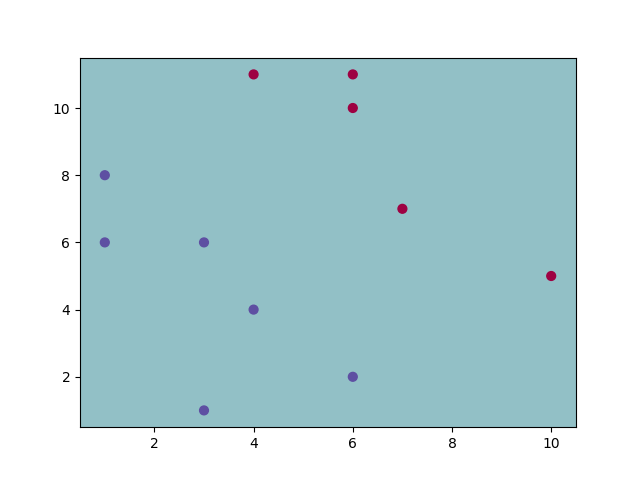
\includegraphics[scale=0.5]{images/run_part1}
	\caption{\emph{run\_part1} plot}
	\label{fig:runPart1}
\end{figure}

\section{A Neural Network}
\subsection{ Implement the activation functions}
You can find them inside \emph{activation.py}. I have also implemented the \textbf{Relu} activation function for didactic purpose.
\subsection{Question 2}
\subsubsection{Forward pass}
In order to calculate the forward pass of a Neural Network we need to compute the activation of each layer, $l$, ad use it as input of the next one until we reach the output layer. 

Equation \ref{eq:forwardPass} shows the activation $a$ of layer $l$ for the $j$-th neuron on that layer.

\begin{equation}
\label{eq:forwardPass}
a^l_j = \sigma(\sum_k w^l_{jk}a^{l-1}_k + b^l_j)
\end{equation}

Where $w^l_{jk}$ is the connection from neuron $k$ in the $l-1$ layer to $j$, $a^{l-1}$ is the activation of the previous layer and $b^l_j$ is the bias of $j$-th neuron in the $l$ layer. With this in mind, we can rewrite \ref{eq:forwardPass} in a efficient vectorised form
\begin{equation}
\label{eq:forwardPassVectorized}
a^l = \sigma(W^la^{l-1} + b^l)
\end{equation}

\subsubsection{delta rules}
A Neural Network try to change its weights in order to decrease the error function, $E$. We define $\delta^l_j$ the output error of neuron $j$ in layer $l$
\begin{equation}
	\label{eq:deltaRule_1}
	\delta^l_j = \frac{\delta E}{\delta z^l_j}
\end{equation}
Strictly speaking, $\delta^l_j$, is how much the error function changes by changing the weighted input on that layer. Applying the chain rule, equation \ref{eq:deltaRule_1} becomes
\begin{equation}
\label{eq:deltaRule_2}
\delta^l_j = \frac{\delta E}{\delta a^l_j} \frac{\delta a^l_j}{\delta z^l_j}
\end{equation}
By knowing that $a^l_j = \sigma(z^l_j)$, Equation \ref{eq:deltaRule_2} can be expressed as
\begin{equation}
\label{eq:deltaRule}	
\delta^l_j = \frac{\delta E}{\delta a^l_j} \sigma'(z^l_j)
\end{equation}  

 %
%We define $\Delta z^l_j$ the quantity added to the $j$-th neuron's weighted input in the $l$ layer by the network.
% The new output of that neuron becomes $\sigma(z^l_k + \Delta z^l_j)$ causing a changing by $\frac{\delta E}{\delta z^l_k}\Delta z^l_j$. 
\subsubsection{Derivatives of the weights}
We want to compute $\frac{\delta E}{\delta w^l_{jk}}$. Applying the delta rule
\begin{equation}
\frac{\delta E}{\delta w^l_{jk}} = \frac{\delta E}{\delta z^l_j}\frac{\delta z^l_j}{\delta w^l_{jk}} =	
\frac{\delta E}{\delta a^l_j}\frac{\delta a^l_j}{\delta z^l_{j}}
\frac{\delta z^l_j}{\delta w^l_{jk}}
\end{equation}
\begin{equation}
\label{eq:derivativesWeigthDeltas}	
\frac{\delta E}{\delta w^l_{jk}} = a^{l-1}_k \delta^l_j
\end{equation}
\subsection{Implement the functions forward and backward of the Neural Network class.}
You can find them in \emph{NeuralNetwork.py}
\subsection{Train Network}
\subsubsection{ Split the data into a train set and a test set}
I decide to split my Training set and Test set by a ratio of 80:20. If we choose a smaller train set we may under-train the network, on the other hand we if we shrink the test set we may \emph{overfit}. We created a function called \texttt{get\_train\_and\_test\_data} in \emph{utils.py} that create the two sets with random sampling.
Figure \ref{fig: train_test_set} shows the plot for the train set and the test set. They are created using \texttt{twospirals} using the standard configuration.

\begin{figure}[h]
	\centering
	\label{fig: train_test_set}
	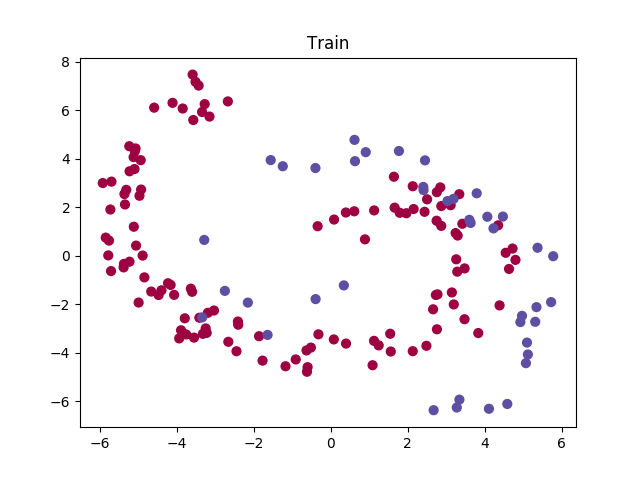
\includegraphics[scale=0.5]{images/train_set}
	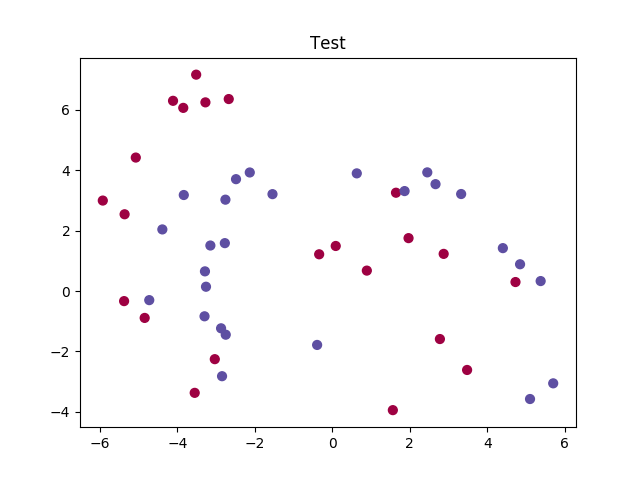
\includegraphics[scale=0.5]{images/test_set}
	\caption{Train set and Test set}
\end{figure}


\subsubsection{Initialise the weights randomly and find a good learning rate to train the network until convergence}
I initialialised the weight using following formula:

$$w = random(n)/\sqrt{2}$$

Where $n$ is the size of the input. This ensures that all neurons in the network initially have approximately the same output distribution and empirically improves the rate of convergence. \footnote{http://cs231n.github.io/neural-networks-2/}

Using $numpy$:
\begin{python}
np.random.randn(in_size,out_size)/np.sqrt(in_size)
\end{python}

\subsubsection{Find a good learning rate}
In order to find the correct learning rate, we decided to fist test the network with different sizes in order have some empirical data. Figure \ref{fig:learning_rate_convergence} shows the convergence rate with five learning rates. The data was generated using the standard inputs and target from \texttt{twospirals} and then normalised the gradient with its average each 100 iterations in order to provide a smoothed line.

\begin{figure}[H]
\centering
\label{fig: learning_rate_convergence}
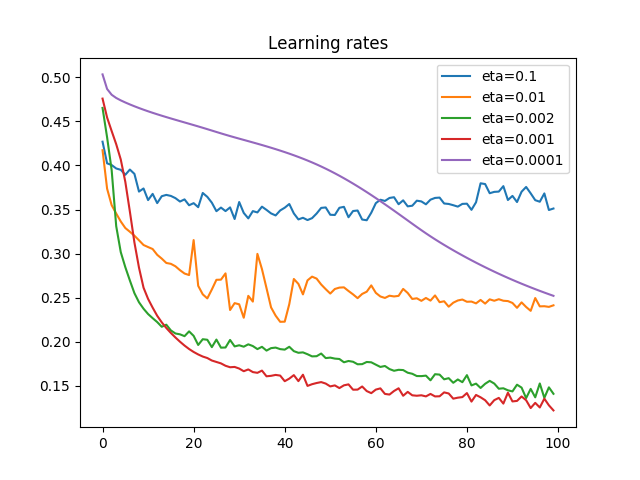
\includegraphics[scale=0.5]{images/NN_eta_vs_training}
\caption{Learning rate convergences}
\end{figure}

This little benchmark shows that a big step size, like $0.1$, do not lead to good converge since it cannot find the correct minimum. On the other hand, a very small eta, $0.0001$, converges very slowly. The best choice is a value between then, $0.002$ or $0.001$.
\subsubsection{Plot the learning rate of at least 5 different learning rates on both sets}
TODO
\subsubsection{Plot the boundary of the model which converged the most on the training data}
Figure \ref{fig: NN_MSE_002_boundary} shows the model boundary after reach a MSE error less than $0.02$ using a step size of $0.002$. The network used the following seed: \texttt{1507986758}
\begin{figure}[H]
\label{fig: NN_MSE_002_boundary}
\centering
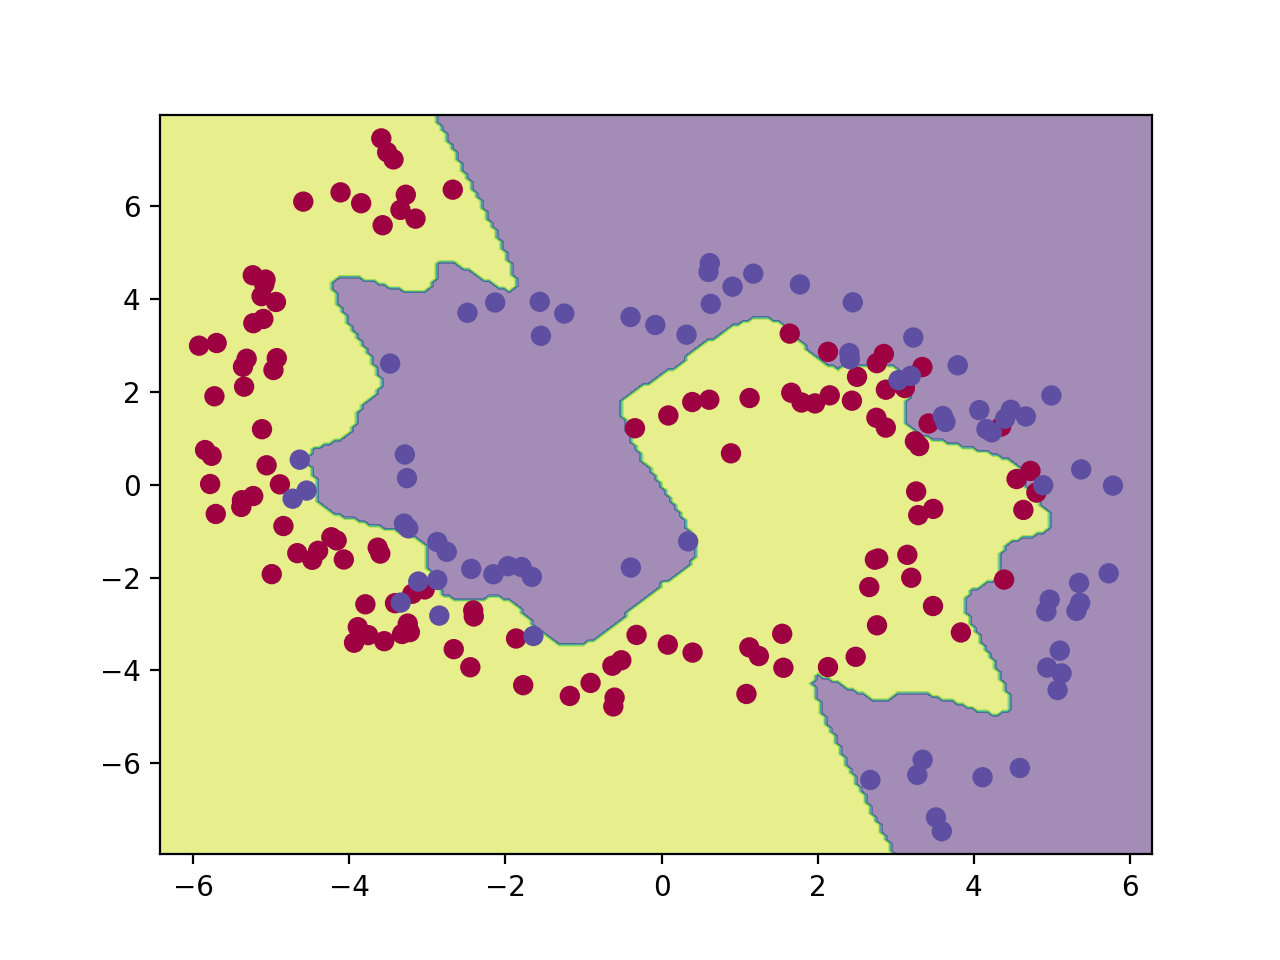
\includegraphics[scale=0.5]{images/NN_MSE_002_boundary}	
\caption{Boundary of the model with MSE less than 0.02}
\end{figure}

\subsection{Explain if this is a good model for the data}

\section{Further Improvements}
In this sections we will analised each extension that I tried to add, even if they did not improve our solution, in order to create a better model.
\subsection{Generic Implementation}
Since the NeuralNetwork class has a fixed number of layers, the first improvement that we did was to create a generic implementation.

The \texttt{BetterNeuralNetwork} class exposes an API that allows to create a generic Neural Network by adding and shaping layers.

After instance the class, is it possible to add a input layer by calling \texttt{addInputLayer(size\_in,size\_out)}. Then the client can add as many hidden layer has he wants by using \texttt{addHiddenLayer(size\_out)}, the "size\_in" is not necessary since it can be easily calculated by the network. Then, as last step, the output layer is added calling \texttt{addOutputLayer(size\_out)}. It follows a full example where we create the same Neural Network from Exercise 2.
\begin{python}
   bnn = BNN()
   bnn.addInputLayer(2, 20, np.tanh, act.dtanh)
   bnn.addHiddenLayer(15, np.tanh, act.dtanh)
   bnn.addOutputLayer(1)
\end{python}

For each layer is also possible to specified the activation function, as default value \emph{signmoid} is used. We have also implemented \texttt{relu} and \texttt{dRelu} to try them.

\texttt{BetterNeuralNetwork} also has \texttt{train} method that performs forward, backpropagation and weight updates directly. It accepts as input the training sets, the targets, learning rate and the momentum flag.
\subsection{Performace}
Due to a better and generic implementation, our \texttt{BetterNeuralNetwork} is slightly faster than the one from Section 2. Table \ref{table: performance_NN_BNN} shows the result of a little benchmark
\begin{table}[ht]
	\label{table: performance_NN_BNN}
\centering
  \begin{tabular}{ | l | c | r |}
    \hline
    iterations & time NN & time BNN\\ \hline
    10 & 17.5ms  & 13.7ms \\ \hline
    100 & 134.5ms  & 128.2ms \\ 
    1000 & 461.6ms  & 458.84ms \\ \hline
    10000 & 4455.6ms & 4157.9ms \\ \hline    
  \end{tabular}
  \caption{}
\end{table}

\subsection{Momentum}
We used Momentum to speed up the convergence of the network, it prevent getting stuck in local minima and pushes the objective more quickly along the shallow ravine. Basically it give a global direction to the gradient descent based on the previous update. Equation \ref{eq: momentum} shows the new update formula. 

\begin{equation}
	\label{eq: momentum}
	\begin{split}
	\Delta w_{ t + 1} = - (\eta \nabla E(w_{t + 1}) + \beta \Delta w_t) \\
	 w_{k + 1} = w_{k + 1} -   \Delta w_{ t + 1}
	 \end{split}
\end{equation}
$\Beta \in [0,1]$ is a the momentum factor, usually between $0.5$ and $0.9$. In our benchmarks we used a classic $0.5$. In Figure \ref{fig:momentum}, we can see the converge rate of a classic gradient descent versus momentum for different step sizes. Momentum converges faster in all cases.
\begin{figure}[H]
\label{fig:momentum}
\centering
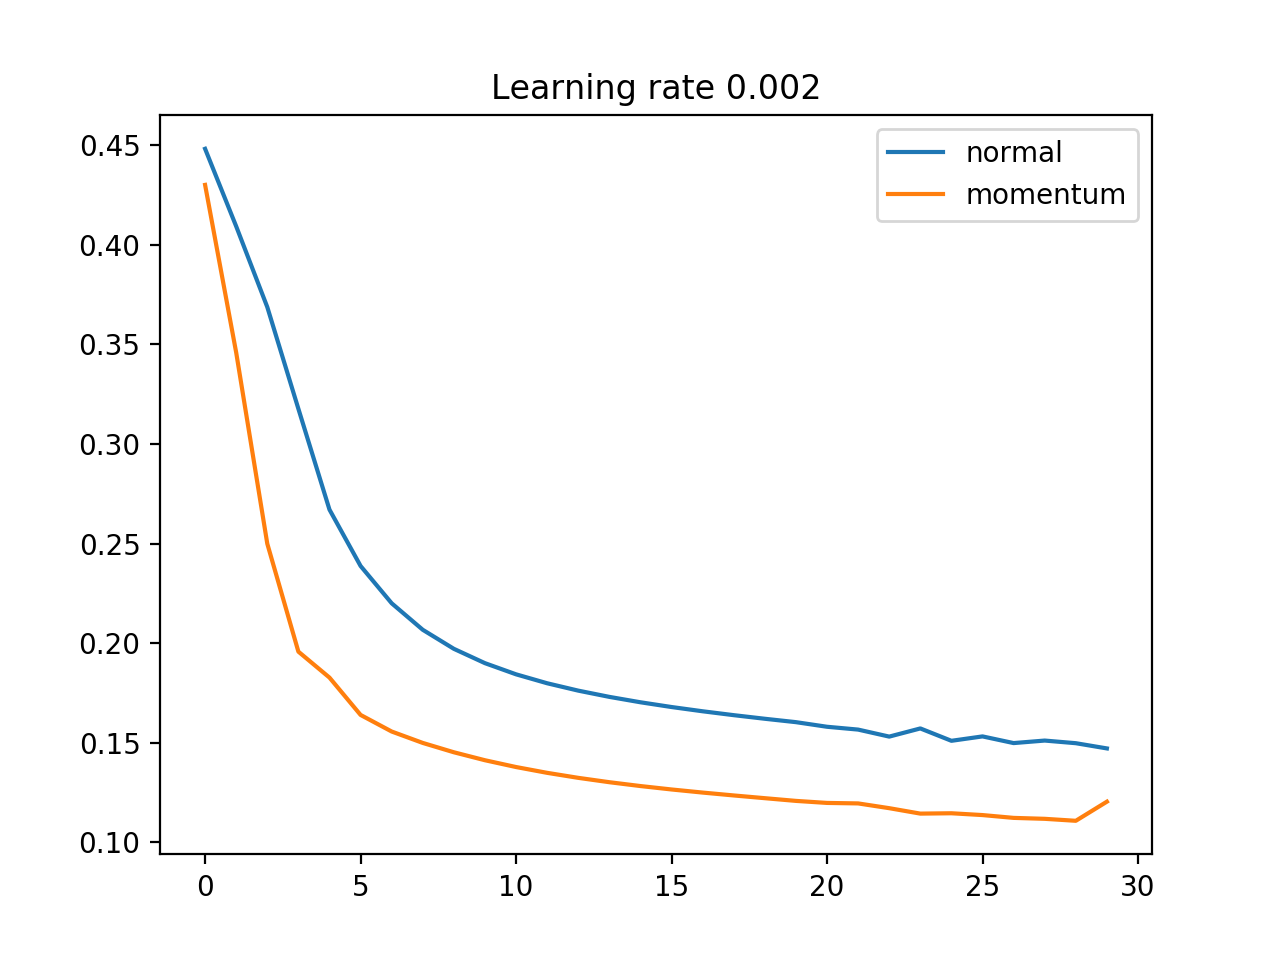
\includegraphics[scale=0.35]{images/momentum_plot_0,002.png}	
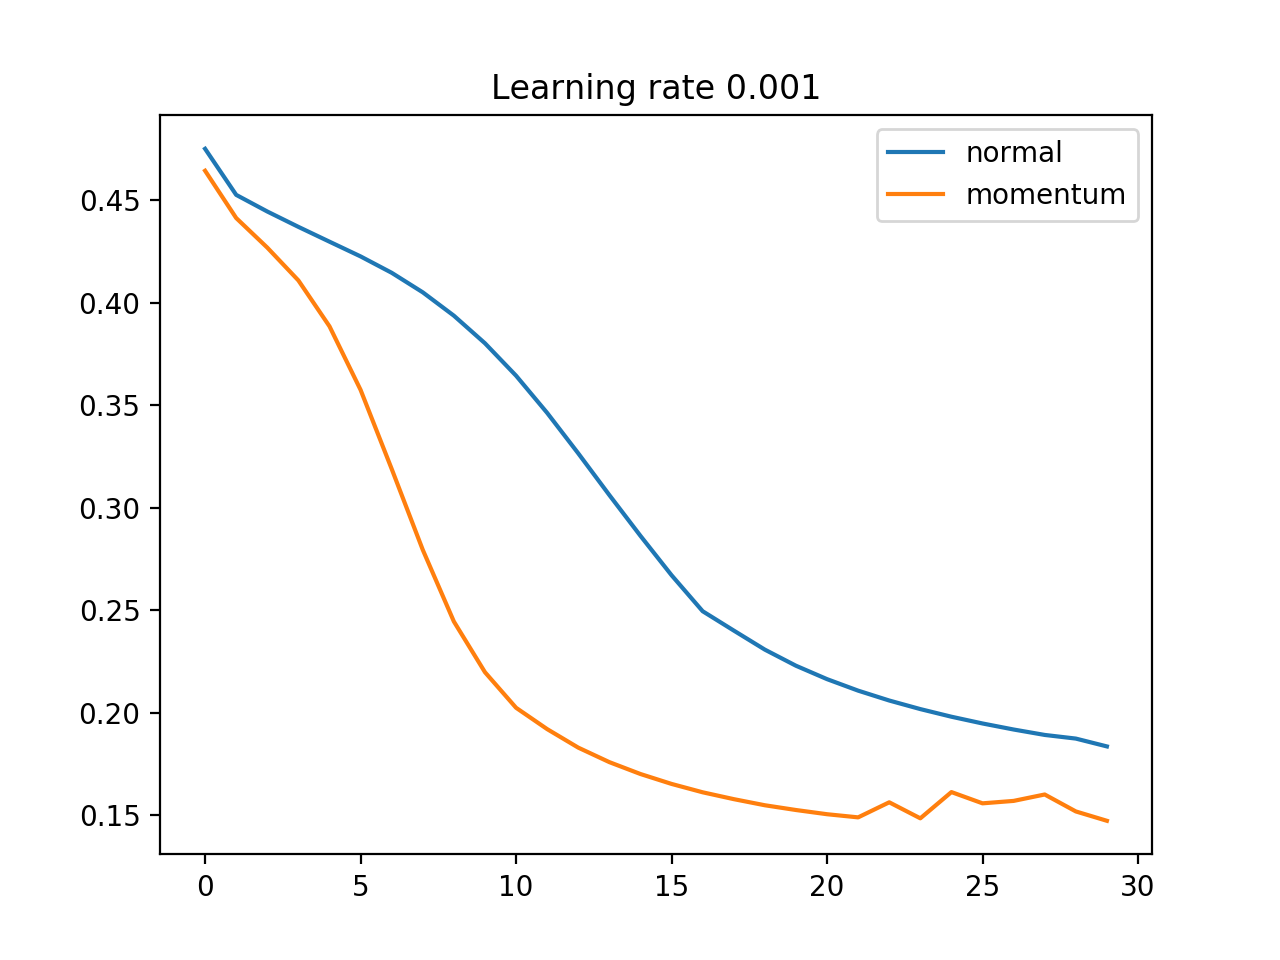
\includegraphics[scale=0.35]{images/momentum_plot_0,001.png}	
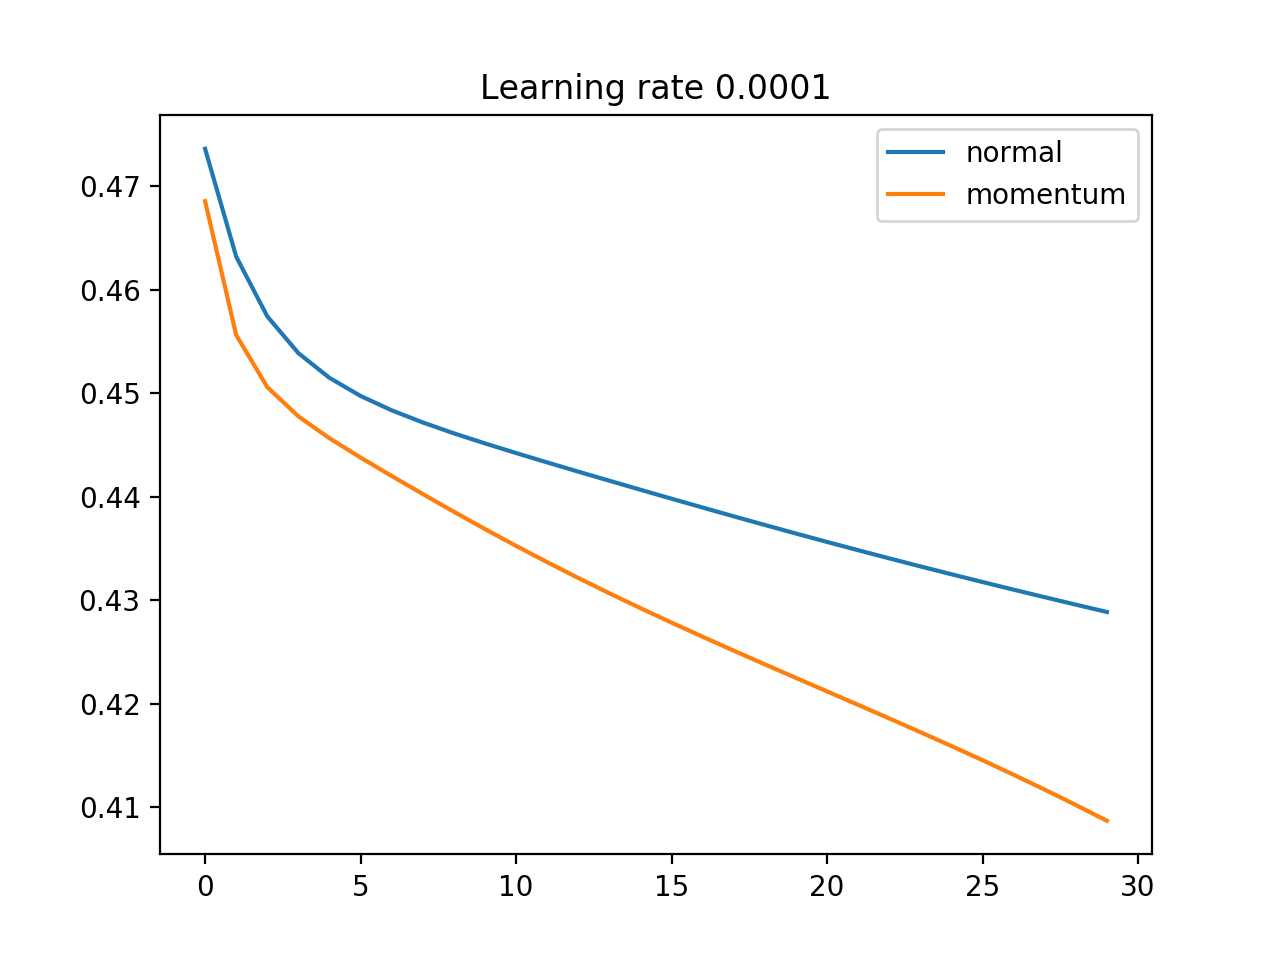
\includegraphics[scale=0.35]{images/momentum_plot_0,0001.png}	
\caption{Gradient Discent vs Momentum}
\end{figure}
In the \texttt{BetterNeuralNetwork} momentum can be enabled by passing \texttt{True} as last parameter to the \texttt{train} method.
\subsection{Dropout}
Dropout is a recently introduced regularisation technique. Basically, each node has a probability to be enable on disable in each forward pass. We implemented it by changing the \texttt{forward} method inside \texttt{BetterNeuralNetwork}
\begin{python}
    def forward(self, inputs):
        self.A = [inputs]
        self.Z = []
        # dropout probability
        p = 0.5
        
        a = inputs

        for l in self.layers:
            z = a.dot(l.W) + l.b
            # create dropout mask
            u = (np.random.rand(*z.shape) < p) / p
            # apply mask
            z *= u
            a = l.activation(z)
            # store
            self.A.append(a)
            self.Z.append(z)

        return a
\end{python}
At each pass, a binary mask \texttt{u} is created and applied to the layer weighted output \texttt{z}. Unfortunately, this approach did not work well for us and lead to a bad convergence.
\end{document}
